\declaration{

%%%%%%%%%%%%%%%%%%%%%%%%%
\chapter*{Candidate Statement of Originality}
I hereby certify that the work embodied in this thesis is the result of original research, is free of plagiarised materials, and has not been submitted for a higher degree to any other University or Institution.
\vspace{4cm}

\noindent
\begin{tabular*}{\textwidth}{%
  @{\extracolsep{\fill}}
  w{c}{3cm}
  c
  w{c}{6cm}
  @{}
}
\signaturedate\today 
&& 
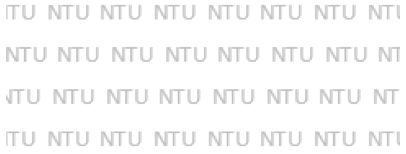
\includegraphics[width=5cm]{class/logos/watermark.png} 
\makebox[0pt][r]{
  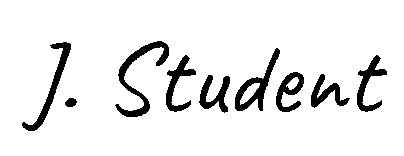
\includegraphics[width=5cm]{Signatures/me.pdf}
}\\
\cmidrule(r){1-1}\cmidrule(l){3-3}
Date && \@author
\end{tabular*}

%%%%%%%%%%%%%%%%%%%%%%%%%%%
\chapter*{Supervisor Declaration}
I have reviewed the content and presentation style of this thesis and declare it is free of plagiarism and of sufficient grammatical clarity to be examined.  To the best of my knowledge, the research and writing are those of the candidate except as acknowledged in the Author Attribution Statement. I confirm that the investigations were conducted in accord with the ethics policies and integrity standards of Nanyang Technological University and that the research data are presented honestly and without prejudice. 
\vspace{4cm}

\noindent
\begin{tabular*}{\textwidth}{%
  @{\extracolsep{\fill}}
  w{c}{3cm}
  c
  w{c}{6cm}
  @{}
}
\signaturedate\today 
&&
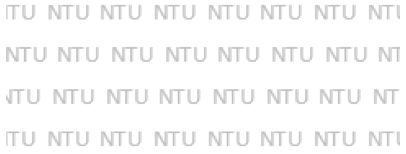
\includegraphics[width=5cm]{class/logos/watermark.png}
\makebox[0pt][r]{
  
\includegraphics[width=5cm]{Signatures/prof.pdf}
}\\
\cmidrule(r){1-1}\cmidrule(l){3-3}
Date && Asst. Prof. First-name Last-name
\end{tabular*}




%%%%%%%%%%%%%%%%%%%%%%%%%%%
\chapter*{Authorship Attribution Statement}

Please select one of the following; *delete as appropriate:

*(A) This thesis does not contain any materials from papers published in peer-reviewed journals or from papers accepted at conferences in which I am listed as an author.

*(B) This thesis contains material from [x number] paper(s) published in the following peer-reviewed journal(s) / from papers accepted at conferences in which I am listed as an author. 

Please amend the typical statements below to suit your circumstances if (B) is selected.

Chapter 4 is published as D.T. Murphy, S. Schmid, J.R. Hester, P.E.R. Blanchard, and W. Miiller.  Coordination site disorder in spinel-type LiMnTiO4.  Inorganic Chemistry 54, 4636-4643 (2015). DOI: 10.1021/ic502747p.

The contributions of the co-authors are as follows:
\begin{itemize}
    \item A/Prof Schmid provided the initial project direction and edited the manuscript drafts.
    \item I prepared the manuscript drafts.  The manuscript was revised by Dr Hester and Dr. Blanchard.
    \item I co-designed the study with A/Prof Siegbert Schmid and performed all the laboratory work at the School of Materials Science and Engineering and the Singapore Synchrotron Light Source.   I also analyzed the data.
    \item All microscopy, including sample preparation, was conducted by me in the Facility for Analysis, Characterization, Testing and Simulation.
    \item Dr James Hester assisted in the collection of the neutron powder diffraction data.
    \item Dr Peter Blanchard assisted in the interpretation of the X-ray absorption spectroscopy data and carried out the spectral interpretation.
    \item Dr Wojciech Miiller assisted in the collection and provide guidance in the interpretation of the magnetic measurement data.
\end{itemize}

Chapter 5 is published as H. V Doan, B. Yao, Y. Fang, A. Sartbaeva, U. Hintermair, V. P Ting, Controlled Formation of Hierarchical Metal-Organic Frameworks using CO2 Expanded Solvent Systems. In press, ACS Sustainable Chemistry \& Engineering (2017). DOI: 10.1021/acssuschemeng.7b01429.

The contributions of the co-authors are as follows:
\begin{itemize}
    \item Prof Ting suggested the materials area and edited the manuscript drafts.
    \item I wrote the drafts of the manuscript.  The manuscript was revised together with Dr. Sartbaeva and Dr. Yao.
    \item I performed all the materials synthesis, collected X-ray diffraction patterns and visible light spectra, carried transmission electron microscopy, and conducted data evaluation.
    \item Dr. Y. Fang conducted the Rietveld analysis of the powder X-ray diffraction data and single crystal structure determinations.
    \item Dr U. Hintermair conducted the molecular dynamics simulations.
    \item Ms. A. Sartbaeva prepared the samples for electron microscopy.
\end{itemize}

\vspace{4cm}

\noindent
\begin{tabular*}{\textwidth}{%
  @{\extracolsep{\fill}}
  w{c}{3cm}
  c
  w{c}{6cm}
  @{}
}
\signaturedate\today 
&&
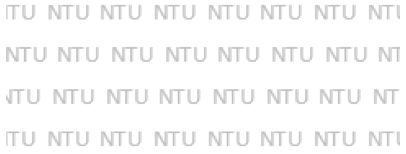
\includegraphics[width=5cm]{class/logos/watermark.png}
\makebox[0pt][r]{
  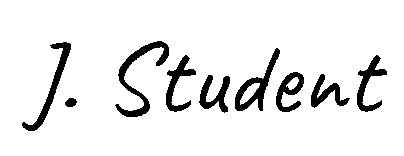
\includegraphics[width=5cm]{Signatures/me.pdf}
}\\
\cmidrule(r){1-1}\cmidrule(l){3-3}
Date && \@author
\end{tabular*}


%%%%%%%%%%%%%%%%%%%%%%%%%%%
\chapter*{Other Publications}
The following list contains other publications conducted during my candidacy on which I was a co-author, but which are not presented in this thesis. (Update this list with your actual publications, not the joke ones listed below).
\begin{enumerate}
    \item M. Adams. The Dead Grandmother/Exam Syndrome and the Potential Downfall of American Society.  Connecticut Review, vol. 12, no. 2, 70--74 (1990).
\end{enumerate}

}